\documentclass[a4paper, 12pt]{article}

%\usepackage{geometry} % Простой способ задавать поля
%\geometry{top=25mm}
%\geometry{bottom=25mm}
%\geometry{left=30mm}
%\geometry{right=30mm}

\usepackage{cmap}                
\usepackage{mathtext}         
\usepackage[T2A]{fontenc}
\usepackage[utf8]{inputenc}    
\usepackage[british]{babel}	
\usepackage{tablefootnote}
\usepackage{threeparttable}
\usepackage{threeparttablex}
%\usepackage{Biblatex-GOST}
%\usepackage{forest}
\usepackage{qtree}

\usepackage{geometry} % Простой способ задавать поля
\geometry{top=25mm}
\geometry{bottom=25mm}
\geometry{left=35mm}
\geometry{right=20mm}

\usepackage{euscript}     % Шрифт Евклид
\usepackage{mathrsfs} % Красивый
%матшрифт
\usepackage{amsmath}
\usepackage{systeme}
\usepackage{setspace}
\onehalfspacing
\usepackage{lscape}

%%% Работа с картинками
\usepackage{graphicx}  % Для вставки
%рисунков
\graphicspath{img/}  %
%папки с картинками
\setlength\fboxsep{3pt} % Отступ рамки
%\fbox{} от рисунка
\setlength\fboxrule{1pt} % Толщина линий
%рамки \fbox{}
%\usepackage{wrapfig} % Обтекание
%рисунков и таблиц текстом
\usepackage{grffile}

\usepackage{csquotes}
\usepackage[style=apa, sorting=nty, bibencoding=utf8]{biblatex}
\addbibresource{citations.bib}
\DeclareLanguageMapping{british}{british-apa}

\usepackage{hyperref}

\title{Blame attribution in autocracies}

\begin{document}
    \thispagestyle{empty}
\begin{center}
 \small{ПРАВИТЕЛЬСТВО РОССИЙСКОЙ ФЕДЕРАЦИИ \\
\vspace{4ex}
  ФЕДЕРАЛЬНОЕ ГОСУДАРСТВЕННОЕ АВТОНОМНОЕ ОБРАЗОВАТЕЛЬНОЕ \\
  \vspace{2ex}
  УЧРЕЖДЕНИЕ ВЫСШЕГО ПРОФФЕСИОНАЛЬНОГО ОБРАЗОВАНИЯ \\ 
  \vspace{4ex}
  «НАЦИОНАЛЬНЫЙ ИССЛЕДОВАТЕЛЬСКИЙ УНИВЕРСИТЕТ \\
  \vspace{2ex}
  ВЫСШАЯ ШКОЛА ЭКОНОМИКИ»}
 \vspace{8ex}
 
 \normalsize{\textbf{ФАКУЛЬТУТ СОЦИАЛЬНЫХ НАУК \\}}
 \normalsize{\textbf{ДЕПАРТАМЕНТ ПОЛИТИЧЕСКОЙ НАУКИ \\}}
\end{center}
\vspace{10ex}
\begin{center}
 НОВИКОВ ВЛАДИМИР АЛЕКСЕЕВИЧ \\
 \vspace{4ex}
 \textbf{АТРИБУЦИЯ ОТВЕТСТВЕННОСТИ В АВТОКРАТИЯХ}\\
 \vspace{4ex}
 \textbf{BLAME ATTRIBUTION IN AUTOCRACIES} \\
 \vspace{4ex}
 КУРСОВАЯ РАБОТА \\
 ПО НАПРАВЛЕНИЮ ПОДГОТОВКИ 41.03.04 ПОЛИТОЛОГИЯ \\
 СТУДЕНТА ГРУППЫ №181 (ОБРАЗОВАТЕЛЬНАЯ ПРОГРАММА «ПОЛИТОЛОГИЯ»)
\end{center}
\vspace{10ex}
\begin{flushright}
 \noindent
 НАУЧНЫЙ РУКОВОДИТЕЛЬ:
 \\
 КАНД. ЭКОНОМИЧЕСКИХ НАУК, ДОЦ.
 \\
 ЗАХАРОВ АЛЕКСЕЙ ВЛАДИМИРОВИЧ
\vspace{2ex}
\end{flushright}

\begin{center}
 \vfill
 МОСКВА -- 2020
\end{center}
	\newpage
	\setcounter{page}{1}
    
    \tableofcontents
    
    
    \section{Introduction}
    
    Why does authoritarian politics persist? This seemingly simple question was asked and answered multiple times, the consensus is still far. Most remarkable examples of long-living autocracies, both the recent and the historical ones like Mexico under the IRP rule, Vladimir Putin's Russia, China in the around last 30 years, and Turkey, are connected with some kind of institutionalization, specifically the electoral institutions \parencite{votingforautocracy, shedler, institutions}. Nevertheless, the strategic interactions of inner regime actors are subject of interest for the researches \parencite{officialmanipulates, morethanwin}, there is still a lack of a universal basic formal model that explains the electoral fraud as the derivative of inner-regime actors incentives.
    \\\\
    This paper aims to contribute to this topic and give one more potential answer to the question raised above. I am combining developing nowadays
    blame attribution and blame avoidance theoretical approach (examples of both theoretical and empirical analysis in this field are provided by \cite{Hood2009, Bovens2007}) with mainstream political science theory on electoral autocracies (approach is based on \cite{competition, shedler}) to provide a slightly different and innovatory point of view on this problem. Specifically, I aim to show how the blame avoidance and the blame minimizing game within inner regime actors shapes  authoritarian politics. For these purposes I establish a formal model of statistics falsification, specifically by the example of electoral fraud, to show how the elections could be won and the regime stays stable, no matter what are the real preferences of the people. The models describe how both the central government apparatus and the regional appointed officials can find a stable equilibrium that allows the long-term regime existence. These results can explain the persistence of authoritarian politics on cases of Mexico's IRP or Putin's Russia which would be discussed below.
    \\\\
	\noindent Concept of blame attribution basically stands for public attribution of responsibility (and blame as the consequence of responsibility) for government performance. As a topical example: the government didn't manage coronavirus outbreak well, and then people know that the government is responsible for the spread and blame their leader. But as far as the leader's reelection depends on his popularity within the people, he tries to avoid attribution of responsibility towards himself using different strategies. For example, the leader can just formally assign this task to his officials and local governors \parencite{putincorona}, or he can blame China as coronavirus pandemic started there \parencite{trumpcorona}. These are basic blame avoidance strategies: blame diffusion, as a feature of the nontransparent system (if it is not clear who is responsible for the decisions, it is not clear whom to blame), and the basic blame shift by public accusations of other actors. In this paper I concentrate on the inner regime blame avoidance, i.e. there are no external actors in the model who can be blamed. So as I focus on the attribution of responsibility within the state: between different levels of power it means an allocation of responsibility between them and thus the task of blame avoidance for the autocrat is to shift the blame towards the lower-level official.
	\\\\
	\noindent Such a study is relevant nowadays. As we can see in a very recent report by Varieties of Democracy project \parencite{vdem} so-called <<third wave of autocratization>> is the trend in most parts of the world, even in Europe and North America. And most newer born autocracies are electoral ones, as in their <<transit>> from democracies. The new paper by \parencite{newway} also studies this topic of newer born competitive regimes, which are products of autocratization and were electoral or even liberal democracies before. As elections in these regimes are mostly kind of <<swayed>> as Levitsky and Way call it democratic elections, regime manipulates electoral process but not shutting it down. Also, as the kind of democratic heritage, these newer born autocracies are dependent on public opinion as they are still dependent on election results and are not closed autocracies yet. That is why my analysis should be relevant for understanding these regimes current and potentially future condition if the trend for autocratization continues.
	\\\\
	\noindent As it was mentioned above, my aim is to look at (potentially rigged) elections in autocracies from point of view provided by theories of blame attribution and avoidance, so that decisions of inner regime actors in the electoral game will be derivatives of the blame game behind them. The innovations in my work are the following: unlike the common tradition in authoritarian studies \parencite{nested, dem1} I will not research regime as one single collective unit, but rather concentrate on inner regime relations between the autocrat and the appointed official (however the second one is still kind of the collective unit) and the public would be more like a technical player rather than a strategic one. My motivation is that study of the game between the regime at large and the people at large means too much generalization and abstraction level and is not really fruitful. Secondly, and it is a consequence of blame avoidance theory -- separation of the autocrat and the appointed official creates the possibility to model the blame game between them. I argue that it may be the case that the distribution of blame between the different levels and actors of the regime will affect their strategies during the election game. The puzzle here is which strategy would be the optimum for the actors: self-blame avoidance or survival of the regime at large, and how can this optic explain the persistence of authoritarian politics, i.e. how stable would the equilibrium be.
    
\section{Existing research and theoretical framework}

    \noindent Both blame attribution theory and electoral autocracies are widely researched. The reasons why autocracies provide elections and how they affect the regime is one of the most developed fields in political science in the post-Cold War era. The most studied evidence is the survival and economic performance of the regime \parencite{inst1, inst2, econorigin}. Baseline's idea is that economic prosperity increases the costs of the potential revolt for the people and thus prevents it. Besides, it provides resources for cooptation or repression, as basic regime survival strategies. Potential outcomes of the elections game in autocracy were also researched, however, scholars' findings still vary between democratization and the stabilization of the regime \parencite{stab2, dem2}: based on specific inner regime conditions and external factors both democratization and survival are possible results.
	
    \subsection*{Why autocracies provide elections?}
	\addcontentsline{toc}{subsection}{Why autocracies provide elections?}
	After about 1991 and collapse of the socialist regimes, the new type of non-democratic regimes came to the focus of scholars: non-democratic regimes with democratic institutions, which are not a \textit{facade} ones, but the real arenas of competition, as they are defined by \cite{competition}. So, it is important to define the conceptual frame field I am working with. First, I am working with a concept of electoral authoritarian regimes \footnote{I use concepts of electoral/competitive authoritarianism/autocracy interchangeably}. It means that the regime that I model has actual working regular elections, however, it can manipulate them in multiple ways. The main question right now is one pulled up in the header. The logic is described by \cite{shedler}.\\\\
	\cite{institutions} suggest, that democratic institutions basically help the authoritarian regime to survive for a longer time, and as the main motivation of any political form is survival, it is an important motive. However, the level of institutionalization might be just fitted, as over- or under-institutionalized regimes do not last as long. How institutions help autocrat to survive? First, "they neutralize threats from below the regime", second, they help to coopt and limit elites. The most important point for my paper here is the neutralization of risks from outside the regime: if people can vote, it is less likely they would revolt. So elections institutionalize people's blame (it will be discussed further).\\\\\
	One more important point is discussed by \cite{parties_elections} who write that elections in autocracies may be helpful for the autocrat to gain information from below: as a ruler can never fully believe their appointed officials, they need somehow to control them, but due to informational constraint and so-called "dictator's dilemma," they have no alternative sources of information. And that is why dictators need elections: to reveal real preferences of population and estimate the quality of elites and officials. Similar ideas of threat from informational constraints are developed by \cite{Kuran} and his concept of "falsification of preferences": he writes, that in autocracies both elites and people prefer not to reveal their real beliefs and that informational vacuum is a double-edged sword. It helps dictator to keep people uncertain about the real state of the world and thus people do not act, because they do not know if anybody shares their protest attitude. At the same time, the dictator himself struggles from it, as he does not know anything about his real support in the population. And that is why elections matter, as they help to reveal preferences of the population.\\\\
	However, elections in autocracies are always a risky game and a trade-off between gaining information and actually staying in power and winning elections. Democratization through elections is always a possible outcome if dictator will not steal results and cancel elections, but that is mostly the case not for hybrids, but for strict autocracies. So it is always game across the outcome of election \cite{nested}. So regimes are often trying to manipulate elections somehow, both before and after them. The more "smart", if we can call it this way, manipulations are done \textit{ex-ante}, as they can help the regime to set the game the way they want it to be played, however, it is always a double-edged sword, as it is studied by \cite{info_elect_change}.\\\\
	But still, as \cite{manipulation} writes, it is important to remember, that elections in autocracies play a different role than in a democracy, mainly because of institutional constraints, created by the regime, and both elections and the regime became something different. To sum up, elections in autocracies are not just a "smart" instrument of manipulation, but a two-sided phenomenon.  the ability to deal with it, as study \cite{stab1} is an important part of survival strategy.
	
    \addcontentsline{toc}{subsection}{Government performance, economic voting and blame attribution}
    \subsection*{Government performance, economic voting and blame attribution}
	And, as mentioned above, elections are elements of uncertainty in political systems. Mainly due to sometimes unpredictable results. However, there are models, that predict electoral behavior, and some of them give evidence on what ruler might do. Mainstream frame nowadays is economic voting, that connects the regime's (economic, but not exclusively) performance and electoral behavior: people punish the regime for bad performance. As in this paper I work in this frame, let review this approach.  The key ideas, described above have empirical evidence though \cite{econ_vote2}, however, the approach itself is controversial. It is not clear how and why people should follow this logic. Still, it is probably the best way to model electoral behavior and it follows basic political and economic logic, and that is why it is so popular, write \cite{econ_vote1}.\\\\
	Blame attribution concept came from economic voting theory and provides an interesting finding that blame attraction by concrete actors differs significantly in the clear and unclear situation of responsibility \parencite{econvote_polit}. It means that if the public does not know who is responsible for the performance it is harder to address blame towards the right actor, which helps the incumbent to diffuse responsibility and lose fewer votes on the election. And the clarity of the responsibility is, in turn, the derivative of the institutional structure of the government (and sometimes circumstances): bicameral systems, i.e. federations, minority or coalition government significantly reduce the incumbent loss of votes as \cite{econvote_polit} empirical analysis shows. In basic models voters' motivation is based on punishment of officials, but before the punish there is blame -- voters need to know \textit{who} to punish. In democracies, the attracter of blame is the current leader and it works clear, as it is described in the paper by \cite{attributionpre}. A similar approach is studied by \cite{blame_gov}, this paper on large empirical data from European elections studies this phenomenon. Also, interesting work is done by \cite{blame_turn}, who shows that bad economic performance mainly affects the turnout itself, which means a higher level of politicization and potential instability of regime. But how would this concept work in the autocracy, where it is mostly unclear whom to blame? \cite{developing} do research how theory applies to developing countries and finds, that lack of informational capacity of the regime can be crucial, as such regimes are mostly not supported enough for economic achievements, but are blamed enough. At the same time, \cite{post-soviet} write, that regime can manipulate public opinion and force "rally round the flag" rather than blame. A combination of the theoretical frame and empirical analysis of the situation with clear responsibility is provided by  \cite{Hood2009, Hood2016} on cases of public exam system failures in Scotland and England in 2000 and 2002. They provide time-series data analysis of blame towards officials in media (by day) and how blame avoidance strategies affected it. Their finding is that politicians are limited in their ability to prevent <<firestorm>> in media by active <<intervention>> strategy and it seems that the optimal strategy for the officials would be the presentational strategy, i.e. public excuses, basic problem admission and public attitudes affection. 
	
	\subsubsection*{Blame attribution and avoidance in non-transparent systems}
	As it was mentioned above, people need to know who is responsible for the performance, and that is why blame attribution works differently in complex and delegated structures and organizations. These are developed topics in public administration theory and blame politics. Here the important distinction is drawn between senior executives and service providers \cite{complex}, he also separates preventive and reactive blame avoidance strategies and tests it empirically on the case of the Berlin transport crisis. Large research on international bureaucratic structures was done by \cite{Rittberger2017, Bovens2007} on European Union structures and Hurricane Katherine case. And that analysis of blame avoidance politics in autocracies, which mostly have less transparent political systems than democracies, this approach might be fruitful. Complex structures with unclear responsibility and division between senior executives and service providers were also studied \parencite{Moynihan2012} on cases of complex delegation structures and international organizations. The results show that in such cases public blame can be attributed due to pre-fiasco reputation or simply would not be personalized at all, for example, EU institutions are blamed for crises, not concrete actors.
    \\\\
	However not many articles were devoted to blame attribution and avoidance in autocratic regimes, which differ from democracies as elections can be rigged and thus elections results are not trustful, as well as state statistics and media. A recent paper by B. Magaloni and S. Williamson \parencite{legislaturesandblame} seeks to fill this gap, as they focus on how legislatures help dictators to relieve responsibility. They prove empirically, on data on African and Asian authoritarian regimes, that legislatures (no matter if they are controlled by ruling majority or not) shift the public blame away from executive power and the autocrat himself. Similar results were empirically proven on data from large Russian cities with appointed or elected mayors \parencite{autocblame}, who found that the ruling party is more often punished for poor economic performance in cities with appointed rather than elected mayor. This topic was also studied on Chinese local level election \parencite{chinablame} with similar results reported: elected officials and country leaders from national minorities are less likely to be replaced during the election rather than appointed officials from the ruling party of the national majority. Still, these papers are based on electoral data, reported by authoritarian regimes, and thus the election could be rigged (and data falsified), and that is the field that this paper tends to contribute in.


    
    \addcontentsline{toc}{subsection}{Center and lower-level officials}
	\subsection*{Center and lower-level officials}
	And here we come to the important and developing nowadays the idea of information control, which is developed in the recent paper by \cite{inform}. They model how the ability to control information and thus ability to attribute the blame affects regime survival. However the model is interesting, it still loses the other way of thinking: the regime is not only a provider of information, but also a recipient, and that is why it needs elections. An illustrative case is researched by \cite{vietnam}. This paper on the case of Vietnamese parliament elections studies noted above trade-off between information, that central apparatus want to gain and the probability of winning elections, and regime solves this with large \textit{ex-ante} manipulation and specific candidate distribution between different electoral areas. That allowed the central apparatus to take information about blame attribution between the local and central levels. Also, we can see research on a quite similar idea in the paper by \cite{china}. The author studies how local level elections in Chinese villages give people the chance to <<punish>> appointed by the central partisan apparatus officials. But the important point is that the central partisan apparatus itself is not blamed in this model, and that is what makes the system stable. To sum up this discussion, the paper by \cite{power_sharing} studies different regime strategies of survival, and the most interesting idea for us is that regime needs the actual power-sharing.
	Another option is studied by \cite{russianregons} who discover that financial transfers to region budgets depend on voters turnout and overall elections result, as the central government provides better financing to regions that show more support. It gives regional authorities different incentives -- to falsify election results in order to gain bigger transfers. The same empirical and theoretical evidence from Russian regional elections were proved by Golosov \parencite{golosov}: the federal center uses electoral data as a KPI for the local governor. Gandhi argues a similar claim on empirical data from Chinese local level elections \parencite{localfraud}. \textit{Facade} local level autonomic institutions do not work, and that is why dictators provide actually working institutions and that is the difference with democratic institutions in democracies.
    \\\\
		\noindent Hereby, as I am studying the specific type of the electoral authoritarianism, the list of all the specific conditions and assumptions is below:
	\begin{enumerate}
	    \item \textit{Regime provides elections} (as its survival is based on <<legitimacy>> strategy or because it uses it as a stabilizing tool \parencite{stab1});
	    
	    \begin{enumerate}
	        \item however \textit{elections can be rigged} by the regime actors at different levels \parencite{manipulation};
	        
	        \item but \textit{regime is not closed} enough to use brutal force and just shut down elections at all;
	        
	    \end{enumerate}
	    
	    \item I concentrate on regimes that depend on public opinion and are minimizing blame as the priority task, or so-called \textit{<<informational autocracies>>} \parencite{inform}.
	    
	\end{enumerate}
	\noindent To sum up the theoretical part: blame attribution in autocracies and democracies is various due to different institutional shape, as to remain in the seat of appointed rather than elected official depends on dictator's will, not the popular vote. Thus the political system is nontransparent and it is not clear for an external observer who is responsible for policy decisions, and thus the task of allocation of responsibility would be not clear. One more rather problematic nuance are blame avoidance strategies of regime actors: while it is more or clear that the autocrat is shifting blame away from himself towards the appointed official, what should be the strategy of the official is yet to be examined. And the game goes around the election as statistical information in autocracies as well as public preferences are unreliable and thereby the election serves the autocrat as the way to gain more trustful information about the true preferences of the people.

    \section{The model}
    \noindent So in this paper my focus is the electoral game inside the regime, specifically around the falsification of the election results. As an autocracy I am studying is an informational one, it means that regime is focusing on information control, i.e. trying to gain as much information about people and their preferences and opinion (specifically opinion about regime itself) as possible and also not allow the public to have information from inside the regime about specific intraregime relations and responsibility \parencite{inform2}. To sum up, inner regime actors (in my model \textit{the autocrat} and \textit{the official}, appointed by the autocrat) are minimizing blame attributed towards them under the condition of staying in power.\\\\
    \noindent Thereby for the autocrat it is the way to know if his appointed official is good enough, for the official the task is to stay in office by providing potentially falsified election while the people are trying to improve the quality of government by showing their preferences at the election.
    
    \addcontentsline{toc}{subsection}{The blame game without blame limitation}
    \subsection*{The blame game without blame limitation}
	There are two strategic players: the autocrat, the official, and the people -- a technical player. The autocrat and the official have qualities denoted by $q_a$ and $q_o \in [0,1]$, respectively. 
    The public observes total quality which is mean of $q_a, q_o$, and does not know separate qualities. The official's quality is his private information; the autocrat believes it to be a random variable uniformly distributed on [0,1]. The autocrat's quality is known to the official.\\
	The timing of the game is as follows:
	\begin{description}
	    \item[$t = 0$:] {\textbf{The nature} randomly chooses quality of the autocrat and the official: $q_a, q_o$ uniformly distributed $\in [0,1];$, which are independent variables}
	    %And it means also total quality of government and blame $q_t = mean(q_a, q_o), b_{t0} = 1 - mean(q_a, q_o), q_t, b_t  \in [0,1]$;
	    
	    \item[$t = 1$:] { \textbf{The public} observes the total quality of government $q_t = (q_a +q_o) /2$ and \textbf{votes}, the people's vote if the function from blame $v_p = 1-blame_t$. Whereas $blame_t = 1 - q_t$; the people's vote $vote_p$ is known by the people and observed by the official, but not by the autocrat.\\
	    \textbf{The official} observes $q_t$ and $vote_p$ and \textbf{chooses} whether to \textbf{steal the election} or not: if the election was stolen $vote_r = vote_p + fraud$, $vote_r$ is published and becomes a public information;\\
	    $fraud \in [0,1]$ is basically the share of votes that were stolen;}
	    
	    \item[$t = 2$:] {\textbf{The autocrat's turn}. He observes $v_f$. If the election was lost $vote_{reported} < 0.5$ the autocrat can either \textbf{give up power} which will end the game or \textbf{annul election results}, thereby addressing the blame towards the autocrat himself.\\
	    Regardless of the vote, the autocrat \textbf{chooses if he replaces the official} or not. If the official was removed the blame declines, so $\Delta blame_t, \Delta blame_a < 0$.}.
    
	\end{description}
	
	\noindent In this game the autocrat is minimizing the blame towards himself and maximizing overall quality of government under condition of staying in power:
	\begin{center}
	    $U_{auto} = \begin{cases}
        q_{total} (1 - blame_{auto}) &  \textbar  \textit{stays in power}\\
        0  & \textbar  \textit{loses power}
	    \end{cases}$
	\end{center}
	%$$U_{auto} = \systeme*{ 1 - blame  \textbar  \text{stays in power}, 0  \textbar  \text{loses power}}$$

	\noindent The official's goal is to hold his office:
	\begin{center}
	    $U_{off} = \begin{cases}
        1 &  \textbar  \textit{stays in office}\\
        0 &  \textbar  \textit{loses office}
	    \end{cases}$
	\end{center}
	And people are maximizing quality of government: $U_{people} = q_{total}$\\\\
	\noindent To summarise: the autocrat and the official produce total quality of government $q_t$, which is the mean of their own qualities $q_t = mean (q_a, q_o)$. The public blames government at large $blame_{total}$, based on aggregated quality of governance: blame is the difference between the expected (I set the expectation equal to 1 which is the ideal quality) and actual quality of government $b_t = 1 - q_t$. The initial blame is equally distributed between the autocrat and the official, as the people do not know who is responsible for the government performance (i.e. $blame_{a} = blame_o = \frac{1}{2}blame_{total}$). The public votes in elections according to their blame: $vote_p = 1 - b_t$. And than the official can steal the election and report $vote_{reported} = vote_p + fraud$, where $vote_r$ becomes the public information.
	
	\begin{center}
        Figure 1: the official's decisions tree:\newline
    \Tree[.\textbf{The people vote: }$Vote_{p}=q_{t}$\\\textbf{The official's turn:} [.\textbf{Chooses fraud?} [.Yes $vote_{reported}=Vote_{p}+Fraud>0.5$\\$\Delta Blame_{total}=Fraud$ ]
                [.No $vote_{reported}=Vote_{people}$\\$\Delta Blame_{total}=0$ ]]]
    \end{center}
	
	\noindent If the election was rigged and $fraud > 0$ the people's total blame increases depends on how much the result is falsified: $\Delta b_{total} = fraud = vote_{reported} - vote_{people}$. The blame increases towards both the official and the autocrat, as it is not clear who stole the vote (so $\Delta blame_{a} = \Delta blame_{o}^{new} = \frac{1}{2} \Delta b_{total}$). And in case the autocrat calls off the election results the blame increases towards himself: $b_{a}^{cancel} = 1 - \frac{1}{2}vote_{people}$ as everybody but the regime supporters is against the election cancellation and as system is nontransparent only half of the regime supporters are personal supporters of the autocrat (blame and response are equally distributed between the autocrat and the official). However if the autocrat replaces the official he partially shifts the blame away and decreases total blame: $\Delta b_{total} = -\frac{1}{2} (b_{total} + fraud)$, so: $$b_{total}^{final} = 1 - vote_{people} +\frac{1}{2}(b_{total}+fraud) - \frac{1}{2}(b_{total}+fraud) = 1 - vote_{people}$$
	i.e. only the regime supporters are left. But that also reduces the blame towards the autocrat (as in public opinion he was partially responsible for the fraud) and thus after the official is replaced: $$\Delta Blame_{auto} = \dfrac{1}{2} \Delta Blame_{total} = - \dfrac{1}{4}(b_{total}+fraud)$$
	Additional strict assumption: if that final amount of blame $b_{total}^{final} < \theta$ is lesser than threshold of revolt $\theta$ which for simplicity of the model will be set to $\theta=1$, the regime lasts (i.e. until not everybody blames the regime it lasts). This assumption would be taken into account afterwards.
	
	\begin{center}
    \hypertarget{fig2_1}{Figure 2.1}: the autocrat's decisions tree if the election was lost:
    \Tree[.\textbf{The official reports the final vote: }$vote_{reported}\leq0.5$\\\textbf{The autocrat calls off the election?} [.No [.\textit{The regime gives up power:}\\\textit{Both the official and}\\\textit{the autocrat replaced} ]]
               [.Yes [.\textbf{The autocrat replaces the official?} [.Yes\\$\Delta blame_t=-\frac{1}{2}(b_{total}+fraud)$\\$\Delta blame_a=-\frac{1}{4}(b_{total}+fraud)$\\$(b_t=1-\frac{1}{2}q_t$\\$b_a=\frac{1}{2}-\frac{1}{4}q_t-\frac{1}{4}fraud)$ ] [.No\\$\Delta blame_t=0$\\$\Delta blame_a=0$\\$(b_t=\frac{3}{2}-q_t+\frac{1}{2}fraud$\\$b_a=1-\frac{1}{2}q_t)$ ] ] ]]
    
\end{center}
	
    \noindent The condition of staying in power for the autocrat is either if the election was won and the blame is lesser than threshold of $\theta$:
	\begin{center}
	    $\textit{the autocrat stays in power} =  \begin{cases}
        vote_{reported} > 0.5\\
        blame_{total} < \theta
	    \end{cases}$\footnote{The second condition is not used in the baseline model}
	\end{center}	
	\noindent Whereas $vote_{reported}$ is a public information. The official loses office either if the autocrat loses power or chooses to remove the official. Let determine the autocrat's incentives for the official's removal:
	\begin{enumerate}
	    \item Estimated by the autocrat the official's quality $\hat q_o$ is worse than the autocrat expects it ($\hat q_o < 0.5$), so he replaces the official with another one, who is expected to be the better manager;
	    
	    \item The election was lost by the regime (i.e. $vote_{reported} \leq 0.5$) and in order to stay in the power, the autocrat cancels the election results and removes the official trying to shift blame (proof at \hyperlink{fig2_1}{figure 2.1}) towards hired official (which may work under the conditions, described above).
	    
	\end{enumerate}
	\begin{center}
    Figure 2.2: the autocrat's decision tree if the election was won\footnote{Full the autocrat's decision tree could be found in the \hyperlink{app3}{appendix}}:\\
    \Tree[.\textbf{The official reports the final vote: }$vote_{reported}>0.5$\\\textbf{The autocrat estimates the official quality:} [.$\hat q_o\geq0.5=E(q_o)$ [.\textit{The official stays}\\\textit{The autocrat stays}\\$(b_t=1-q_t+fraud$,\\$b_a=\dfrac{1}{2}(1-q_t+fraud))$ ]]
               [.$\hat q_o<0.5=E(q_o)$ [.\textit{The autocrat replaces}\\\textit{the official:}\\\textit{as $\hat q_o < E(q_o)$} [.\textit{The autocrat stays}\\\textit{The official replaced}\\$(b_t=b_t+\Delta b_t=\dfrac{1}{2}(1-q_t+fraud)$,\\$b_a=b_a+\Delta b_a=\dfrac{1}{4}b_t+fraud)$ ]]]
    ]
    \end{center}
	\noindent The autocrat estimates the official's quality from reported election result as follows: $$\hat q_o = 2vote_{reported} - q_a$$ (as the autocrat expects that $vote = q_t = \dfrac{q_a + q_o}{2})$). So the official's task to stay in office is to falsify the election so that the autocrat's estimate of his quality would be greater than 0.5, which is the expected value of the official's quality: as the autocrat expects it to uniformly distributed on [0,1]. Thus the official at his turn aims to falsify the election result so that $$2  vote_{reported} - q_a \geq 0.5$$ i.e. $fraud \geq \dfrac{0.5 - q_o}{2}$ (thus $\Delta b_{total} \geq \dfrac{0.5 - q_o}{2}$). After that the autocrat observes $vote_{reported}$ and acts based on it:
	\begin{description}
	
	    \item[if $vote_{reported} > 0.5$] \textbf{and the election was won}: the autocrat is pleased with the result as he stays in power and tries to maximize the quality of government in order to minimize the people's blame. So if estimated by the autocrat the official's quality is better than (or equal to) the expected $\hat q_o \geq 0.5$ than the autocrat has no motivation to replace the official and game ends, otherwise he replaces the official;
	    
	    \item[if $vote_{reported} \leq 0.5$] \textbf{and the election was lost}: the autocrat calls off the election in order to stay in power, the people's blame towards him increases and the autocrat, to minimize it removes the official\footnote{Which means that the official as the strategic player falsifies election in order to get $vote_{reported} > 0.5$}. And then if blame is lesser than 1 he stays in power, otherwise, regime was changed by revolt.
	    
	\end{description}
	
		\begin{center}
    \hypertarget{fig3}{Figure 3}: outcomes of the game for the official based on the final vote:
    \Tree[.\textbf{The official reports the final vote} [.$vote_r>0.5$\\\textbf{The autocrat estimates the official's quality:}\\$\hat q_o=2vote_{r}-q_a\Leftrightarrow vote_{r}>\frac{0.5-q_o}{2}$ [.$\hat q_o\geq0.5=E(q_o)$ [.\textbf{The official stays}\\\textit{Estimated quality better}\\\textit{than expected} ]]
               [.$\hat q_o<0.5=E(q_o)$ [.\textbf{The official replaced}\\\textit{Estimated quality worse}\\\textit{than expected} ]]]
          [.$vote_r\leq0.5$ [.\textbf{The official anyway is replaced:}\\\textit{by the autocrat (to shift blame)}\\\textit{or due to regime change} ]]]
   
\end{center}
	
	\noindent The results lead us to the following conclusions: the official no matter what is the peoples' vote has incentives to falsify the results so that $vote_{reported} > 0.5$ and $fraud > \dfrac{0.5 - q_o}{2}$: so $fraud > 0$ if $q_o < 0.5$ or $\dfrac{q_a + q_o}{2} < 0.5$ as otherwise the official would be replaced because the autocrat would estimate his quality as insufficient or because the election would be lost and the official removed anyway. In other words, it means that in the nontransparent system the appointed official can only choose \textit{the portraying loyalty} strategy, as his position depends only on how the autocrat estimates the official based on the election results.
    \\\\	
	\noindent At the same, time the autocrat himself plays \textit{the personalistic} strategy since he cares about his personal blame avoidance. However, as he is maximizing the overall quality of government (which basically means that he appoints the official with better quality if possible) the autocrat also minimizes the overall blame towards the government: still, the autocrat does not care about the specific official. Nonetheless, the game regardless of initial conditions comes for \textbf{the equilibrium where both the autocrat and the official stay in power} (proof at \hyperlink{app1}{the appendix}).	And for the people, the result means that the total quality of government is not likely to change apart from the revolt and the regime change at large: as the official manages to falsify the results and thus to increase the estimated quality.

    \subsection*{<<Strict assumption>>: blame leads to revolt}
	\addcontentsline{toc}{subsection}{<<Strict assumption>>: blame leads to revolt}
	However, the assumption that $blame_{total} > \theta$ leads to revolt (whereas $\theta = 1$) was mostly excluded from the previous analysis, as I focused on exclusively blame minimizing task. And at this part, I will include the option of revolt into the analysis and analyze how it shapes the results. The timing of the game would be similar and the revolt would be the move of the people at $t = 3$ after the autocrat's turn.
    
    	    	\begin{center}
    \hypertarget{fig4}{Figure 4}: outcomes of the game with blame limitation for the official:
    \Tree[.\textbf{The official reports the final vote} [.$vote_r>0.5$\\\textbf{Estimated quality $q_o$ satisfactory?}\\$\hat q_o=2vote_{r}-q_a$ [.Yes\\$\hat q_o\geq0.5=E(q_o)$\\\textbf{$b_{total}$ exceeds threshold?} No,$b_t<\theta$\\\textbf{Stays} Yes,$b_t\geq\theta$\\\textbf{Replaced}     ]
               [.No\\$\hat q_o<0.5=E(q_o)$ [.\textbf{Replaced} ]]]
          [.$vote_r\leq0.5$ [.\textbf{Replaced} ]]]
   
\end{center}
    
    \noindent Note, that the perspective of revolt would not affect the official's incentives and behavior, as his tenure fully depends on the autocrat's will, not on the people's preferences, so the official's move and strategy stay the same:
	\begin{enumerate}
	    \item if $vote_{people} < 0.5$ he falsifies the election results so that: $fraud > 0.5 - vote_{people}$ and $vote_{reported} > 0.5$ -- in order to win the election and thus stay in office;
	    
	    \item if $\hat q_o < 0.5 \Leftrightarrow vote_{people} - q_a < 0.25$ he falsifies election so that: $fraud > \dfrac{0.5 - q_o}{2}$ and $vote_{reported} > q_a + 0.25 \geq 0.5$ -- in order to overstate his estimated quality and stay in the office.
	    
	\end{enumerate}
	
	\noindent Coming to the autocrat, at the end of his turn total amount of blame can be:
	\begin{enumerate}
	
	    \item $b_{t1} = 1 - q_t + fraud$ -- which stands for the case where the election was won $vote_{reported} > 0.5$ and estimated the official's quality is satisfactory $\hat q_o > 0.5, vote_{reported} > q_a + 0.25$ so the official stays;
	    
	    \item $b_{t2} = \dfrac{1}{2}(1-q_t+fraud)$ -- the case where the election was won $vote_{reported} > 0.5$ but the official replaced (this basically was not the case for the blame minimizing game with no revolt as the official always falsifies election and never is replaced)
	    
	    \item $b_{t3} = 1 - \dfrac{1}{2}q_t$ -- and that is the case where the election was lost and called off and the official is replaced;
	    
	    \item $b_{t4}=\frac{3}{2}-q_t+\frac{1}{2}fraud$ -- finally the never achieved outcome where the election was lost and canceled and the official stays in office. Still, as the autocrat's utility is higher when the official is replaced this outcome is never achieved (proof at \hyperlink{fig2_1}{2.1})
	    
	\end{enumerate}
	
	\noindent Taking the new restriction into account I test the equilibrium outcome with the new limitation. The result is as follows (proof at \hyperlink{app2}{the appendix}):
	\begin{description}
	    \item[ If $q_a > 0.5$] (i.e. the autocrat is competent) the revolt is only possible if the official is absolutely incompetent $q_o = 0$, and can be prevented if the autocrat estimates the total blame and replaces the official (and thus reduces the blame);
	    
	    \item[ If $q_a \leq 0.5$] (i.e. the autocrat is incompetent): the revolt is possible if the official is incompetent too $q_w + q_a \leq 0.5$ and fraud was redundant $fraud \geq 0.75$ (otherwise the official's replacement would reduce blame enough to prevent the revolt).
	    
	\end{description}

    		
	\begin{center}
	    Figure 5: Possibility of the revolt based on the autocrat's and the official's qualities:
	    
	    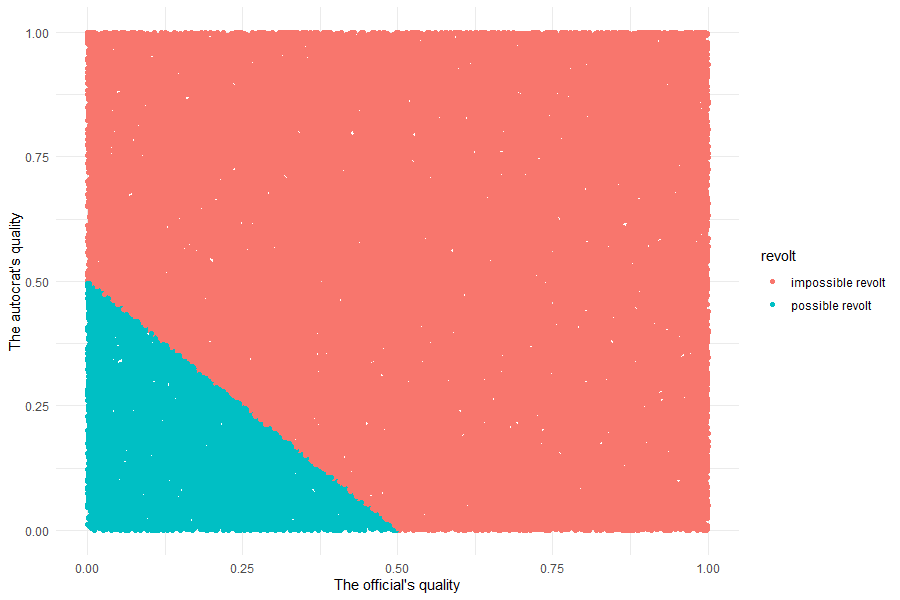
\includegraphics[width=\textwidth]{img/revolt.png}
	    
	\end{center}
	

	\noindent Thereby if at least one of the regime actors is competent (or at least their total quality is more than half of ideal $q_t > 0.5$) the probability of the revolt is equal to zero as the autocrat can reduce blame by replacement of the official. However, the main difference with the baseline model is the increase in the expected total quality of government as there is a possible outcome of the official's replacement with another one with the expected quality of 0.5 (which might be higher than the actual quality). Thus the conclusion for the <<strict limitation>> assumption is that possibility of people's revolt due to excessively high total blame level leads to an increase of total quality of government as the incompetent official would be replaced with a potentially more competent one.
	
	\section{Discussion}
	In this and the following sections the results from the two previous parts are restated and reinterpreted but in the broader context. Also, I would argue if the results are suitable for the explanation of real-life examples of persistent electoral authoritarian regimes.
    \\\\
	\noindent First, if there is no risk of people's revolt (i.e. there is no punishment for the election results falsifications) and the autocrat estimates the official's quality based on the reported election results \parencite{parties_elections}, the official would have incentives to falsify the election results so that the election would be not only won by the regime but so that the final vote would show that the official is more competent than he really is. This model of interaction between the central government and local officials was proved empirically: as federal state may encourage regions with <<good>> electoral results and <<punish>> the regime with <<bad>> results \parencite{russianregons}. Thus this system encourages the local level officials to falsify the elections so that the reported result is satisfactory for the central government \parencite{golosov}. And in this way, the model with no blame restrictions leads to the equilibrium with \textit{<<falsified enough>>} election results whereby all the regime actors (i.e. the autocrat and the official) stay in power and total quality of government is not likely to change. On the other hand, the autocrat cannot get the information about the true preferences of the people -- the autocrat by his own hands constructs the system that makes it harder for himself to gain information about the people, still, he stays in power. To wit, if the people have no direct way to affect policy decisions. As the election is rigged by the moderator -- the official and thus there true preferences are hidden from the autocrat. However, in my models the autocrat is pretty benevolent as his blame minimization utility corresponds with the people's gain for quality of governance.\\\\
	This result is partially explained by the ignorance of <<loyalty-competence dilemma>> of the authoritarian politics: the autocrat has to choose between loyal or competent surrenders as disloyal can arrange a coup against the autocrat and incompetent simply perform worse than expected \parencite{loyal_competent_2}. This game of loyalty-competence also means that the official has to choose his level of loyalty based on his competence \parencite{loyal_competent_1} and the autocrat also chooses between economic performance quality and loyalty warranty. However, I simplify the official's task as his tenure depends entirely on the autocrat's decision and his only strategy is to play the autocrat's game. The autocrat's task is simplified as well as he only estimates the quality of the official, not his loyalty.\\\\
	Nonetheless, the results change as the people's blame can lead to revolt if it is higher than a certain threshold. In this model with blame limitation the revolt is possible for the incompetent the autocrat and the official and this possibility leads the autocrat to blame-shifting and expected quality increasing action: replacement of the official. The results are not encouraging however from the democratization perspective point of view, as there is no robust equilibrium of the regime change. The autocrat mostly manages to reduce blame enough (by replacing the official) to prevent the revolt. Hereby, the results correspond with the theoretically explained and empirically tested persistence and stability of electoral authoritarian regimes \parencite{newway, institutions}. Especially formal model from this paper confirms the empirical findings from recent Magaloni and Williamson paper \parencite{legislaturesandblame}, who claim that multi-level government structure helps the autocrat to shift blame away from the executive power and himself (the paper studies blame distribution between executive and legislative powers).\\\\
	To summarise, the first model can be applied for different kinds of statistical information, which falsification is not crucial for the people. That is to say, it is \textit{the general model of (unrestricted) statistics and preferences falsifications} by the lower-level officials in autocracy. And in that case without the probability of punishment the official falsifies the information and the regime stays stable. Nevertheless, the risk of the people's blame flawing into revolt forces the government for changes, still minor (as the autocrat stays in power). Note also that the official's strategy does not change with the risk of the revolt as he depends on the autocrat's decisions, not the popular preferences. The inference from the second model is that \textit{as long the autocrat is capable of shifting blame away from himself by the replacement of the appointed officials he can stay in power no matter how competent he personally is}.
	\\\\
	However both formal models from this paper face certain theoretical limitations, namely: I disregard possible preassigned blame distribution between the autocrat and the official as well potential media bias, which means I mostly excluded more <<traditional>> ways of blame attribution and avoidance. Still, it was due to the assumption of the non-transparent political system, total exclusion of media from the model is a bit unrealistic. Also, the autocrat does not take into account potential falsification of statistics by the official, which is passable for the non-repeating game, but as an outline for the further development of the model, the autocrat should also estimate the probability of fraud by the official. One more notable point: as blame is the difference between the expected and actual observed quality of government $blame_{total} = E(q_{total}) - q_{total}$ \textbar $E(q_{total}) = 1$, and the government can potentially affect the expectations of governance quality in order to lower it and thus the people's blame so that: $E(q_{total}) < 1 \to blame_{total}^{affected} < 1 - q_{total}$.
	
	\section{Suitability for the actual case study analysis}
	
	\noindent At this part I would discuss how the outcomes of the formal model correspond with the actual state of affairs. I would focus on two notable examples of long-living electoral authoritarian regimes, namely the Mexican Institutional Revolutionary Party regime which lasted for more than seventy years from 1929 to 2000 and the party still exists and the contemporary Russian political regime under the Vladimir Putin rules, which lasts for twenty years until the nowadays.
	
	\subsection*{Institutional Revolutionary Party rule in Mexico}
	\addcontentsline{toc}{subsection}{Institutional Revolutionary Party rule in Mexico}
	IRP rule in the XX century in Mexico is widely researched. One of the most complete sources is "Voting for autocracy" by Beatriz Magaloni \parencite{votingforautocracy}, apart from multiple more narrowly targeted papers \parencite{officialmanipulates, morethanwin, stab2, dem1}. Nevertheless, that kind of regime does not fully correspond with the initial assumptions of the model, namely the regime in Mexico was party-based while the model stands for a more personalistic one. Still, the logic of the model can suit these conditions as \textit{the autocrat} from my model basically could be associated with the central party apparatus, while \textit{the  official} stands for the regional elites. What is more, there is evidence that regional elites under the IRP rule had incentives not only to win elections but also to show that they are effective enough, so that just win was not enough \parencite{morethanwin}. This feature perfectly corresponds to my key initial assumption. So here is how my model can be applied for the analysis: I test how the features of the IRP regime, described by Magaloni, correspond with the model outcomes.
	\\\\
	First, it is a widely known fact that the IRP regime was supported more in the underdeveloped regions of the country \parencite{underdevelop}. This fact suits for my model as the vote and the blame are based on the difference between the actual and the expected quality of governance $vote_{people} = 1 - blame_{total} = 1 - (E(q_t) - q_t)$. Thereby if the region is underdeveloped the expected quality should be lower and thus the lower is the blame and the higher is the vote. Even so, it poses the further question about the dynamic and repetitive game. With the time added, the expected quality of government and quality of life might be constantly growing (as the overall quality of life is growing on Earth is growing), and the quality which was passable at the beginning of the regime might not be satisfactory at the end. On the other hand, the regime can affect the people's expectations, as the quality of governance at time $t-1$ might affect the expectations at time $t$. This is a complicated topic and the outline for the further development of the model.
	\\\\
	Second, even though my model for the purpose of simplicity does not include any kind of direct vote-buying, apart from basic quality of governance, while in Mexico it was a common practice \parencite{vote_buy}. That is a fruitful field for the further development, as the provision of more personalized public and club goods could be recognized by the people as the more personal gift from a concrete actors (this thesis needs he verification so). Which means that a more narrowly targeted vote-buying can serve as a smart instrument of blame avoidance. It can be potentially included into the model as a further feature, as private or club goods provision could be modeled as a part of not the aggregate quality of government, but the official's or the autocrat's own quality.
	\\\\
	Third, throughout the IRP rule, the main rivalries for the regime were primary party members, who have chosen not loyalty but their own ambitions \parencite{members}. Although, as it was mentioned above, I excluded these dimension of the principal-agent interactions from my model, it corresponds with the results as the regime sustainability in my models is rooted in full dependency of the official, which reduced his strategies. If other strategies are available, i.e. if there is the exit option, this alternative strategy should affect the official's behavior and make him at least partially independent, as the official is in different kinds of models \parencite{loyal_competent_1}. Thus my model partly predicts this outcome.
	\\\\
	Finally, IRP was forced to give up power not after a massive fraud in 1988 but after an observed election in 2000, which made the people's voting results the public information \parencite{fraud}. This also corresponds with my model: just the fact of fraud is not enough, there should be the risk of revolt to force the regime to give up power.\\
	To summarise, even though there is no evidence that IRP cared about blame avoidance and the people's blame distribution within the regime, my model can explain the duration of the regime's rule and partially explain the regime's decline.
	
	\subsection*{Contemporary Russian regime}
	\addcontentsline{toc}{subsection}{Contemporary Russian regime}
	The current Russian political regime is yet to be studied comprehensively, however some specific features of authoritarian electoral control in modern Russia were investigated \parencite{golosov, russianregons, post-soviet}. In this way, the available information allows concluding that the regime satisfies the initial assumptions. Russia is an informational autocracy \parencite{inform} and the regional governors kind of KPI is based on electoral results. Thus I can apply findings from my model to the modern Russian political regime.
    \\\\    
	\noindent First, the authoritarian turn in Russian politics occurred and stabilized at the same time the direct elections of regional governors were canceled in 2005. Nevertheless, the coincidence in time does not imply causation, and further empirical tests are necessary to prove how these events are connected, some researchers have studied this topic \parencite{governors}. Still, it perfectly corresponds with the logic of the model: to attempt an electoral control without any concerns the autocrat needs to control the region-based officials. And if the official's tenure depends on the autocrat the only strategy for the political survival the official has is to play the autocrat's game. And that is how the authoritarian politics persists, even though the direct governors elections were returned seven years later, the authoritarian consolidation should happen already (and newer governors elections are not really direct though, so that the governors are more manageable than they were before the reforms).
    
	\begin{center}
	    Figure 6: Liberal democracy (dark blue line) and polyarchy (light blue line) indexes scores for Russia, data from the Varieties of Democracy dataset \parencite{vdem_data}
	    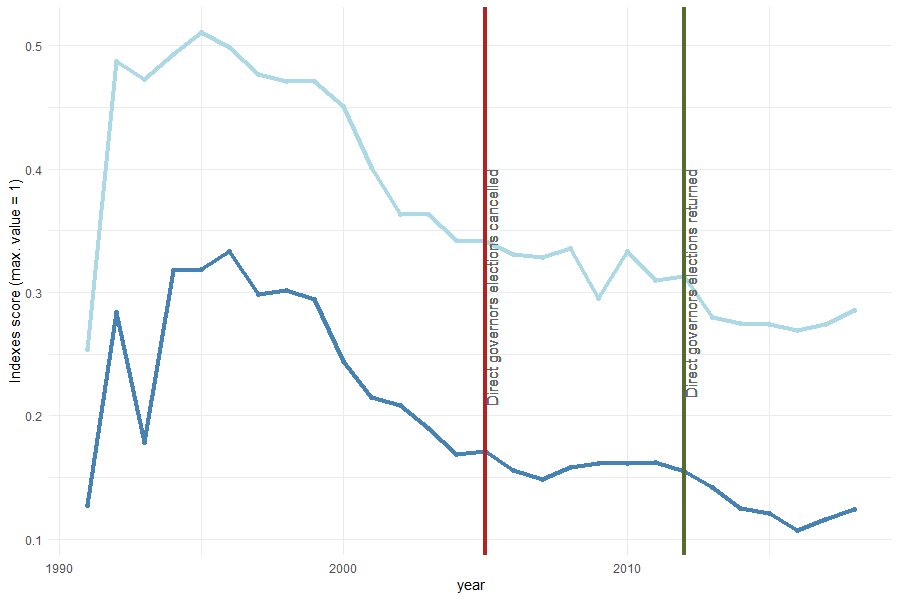
\includegraphics[width=\textwidth]{img/russia_3.png}
	\end{center}
	
	\noindent What is more, in last years there is a tendency that regional governors are hired massively after the unsatisfactory performance or if their popularity is low and they are blamed by the people \parencite{governors2}. The potential logic behind it is the following: as the Russian political system is non-transparent and it is not clear for the people who is responsible for the performance. And as the Russian regime is a kind of personalistic one (at least state media shows the regime this way) the people image of the government is associated with the leader himself. Thus all unsatisfactory performance tends to be at least partially assigned to the leader and to shift the blame away and address it to the local officials the governors are replaced. That is directly the logic of blame avoidance by the autocrat I described in my model: the autocrat replaces the official to shift the blame (and stays in power as long as this trick works).
	\\\\
	To summarize, the general formal model I established in this paper with the addition of some specific features can explain the persistence of at least two long-living electoral autocracies. Yet the "case study" analysis was primitive and far from quality needed for any kind of inference: the more detailed empirical analysis is required. Nevertheless, the basic superficial analysis shows the applicability of the models. However, further development of the model is still necessary, specifically some new features as the competence-loyalty dilemma and media bias, as well as further empirical tests.
	
	\section{Conclusion}
	Why does authoritarian politics persist and especially why electoral autocracies are the most stable ones? How blame attribution and avoidance shape authoritarian politics? How the autocrat gains information about the preferences of the people in the system with non-transparent information flaws? Recent papers in political science are showing that authoritarian persistence can be explained by institutionalization, i.e. power-sharing, (at least partially) meaningful elections, etc. Blame attribution and avoidance in authoritarian politics is also connected with a multi-level government system with unclear responsibility, which also requires power-sharing. Finally, the way the autocrat estimates his appointed officials and different levels of government and gains information are elections, conducted by the lower-level officials. Nonetheless, the existing framework is lacking a more general formal theory of blame attribution and preferences falsification in autocracy.\\\\
	I presented formal models that tackle this problem and show how and why the appointed official falsifies the people's preferences and how the autocrat interacts with his appointed official. The baseline model can be applied for various statistics falsifications, not only for the electoral results, as it has no direct punishment for the falsifications. This game brings the equilibrium with all the upcoming information \textit{falsified enough} by the low-level appointed official. Thus both the official and the autocrat stay in power: as there is no  risk of revolt in baseline model and the official reports the \textit{good enough} statistics to stay in office, which means that quality of government stays the same.\\\\
	The game with the limitation of the affordable blame level brings in the possibility of revolt in case the people's blame reaches a certain threshold. This second model implies that the perspective of the revolt, i.e. there is punishment for the regime for blame overgrowth. The result is that the perspective of people's uprising force the autocrat to replaces the official under some circumstances (namely, if both the official and the autocrat are incompetent). The implication from this development of the former model is that if the falsification of preferences matters for the people so that they are able to revolt, it forces changes in the government policy. That leads to an increase in the governance quality, which satisfies the people, however, the regime change is not likely. That explains the stability of the electoral autocracies under a certain leader, who changes the appointed officials.\\\\
	This is a general formal model that can incorporate further assumptions and limitations. The approach is novel and still developing, future work is necessary on more detailed blame distribution between the actors, the repeating game would be a useful addition too, as well as an empirical test of the results. Still, the model is useful for the understanding of the persistence of authoritarian politics from the blame attribution and falsification of preferences perspective. 
	
	\newpage
	\section{Appendix}
    \addcontentsline{toc}{subsection}{Proof for the baseline model}
    \subsection*{\hypertarget{app1}{Appendix 1}: proof for the baseline model}
    
    \noindent Taking $q_a, q_o = \alpha, \omega \in [0,1]$\\\\
    Thus $q_t = \dfrac{\alpha+\omega}{2}, blame_t = 1 - \dfrac{\alpha+\omega}{2}, vote_t = \dfrac{\alpha+\omega}{2}$\\\\
    Based on \hyperlink{fig3}{figure 3} the only way for the official to stay in office is two satisfy the two following conditions:
    \begin{enumerate}
        \item $vote_{reported} > 0.5 \Leftrightarrow fraud > 0.5 - vote_{people}$
        
        \item $\hat q_o > 0.5 \Leftrightarrow fraud > \dfrac{0.5 - q_o}{2}, vote_{reported} > q_a + 0.25$
        
    \end{enumerate}
    
    \noindent Which means:\\\\
    $fraud = max(0.5 - \dfrac{\alpha+\omega}{2} + \gamma; \dfrac{0.5 - \omega}{2} +\gamma)$ \textbar $\gamma > 0$\\
    $vote_{reported} = \dfrac{\alpha+\omega}{2} + max(0.5 - \dfrac{\alpha+\omega}{2} + \gamma; \dfrac{0.5 - \omega}{2} + \gamma)$\\
    $vote_{reported} \geq \dfrac{\alpha+\omega}{2} + 0.5 - \dfrac{\alpha+\omega}{2} + \gamma = 0.5 + \gamma > 0.5$ \\\\
    $vote_{reported} \geq \dfrac{\alpha+\omega}{2} + \dfrac{0.5 - \omega}{2} +\gamma = \dfrac{\alpha + 0.5}{2} + \gamma$\\\\
    $\hat q_o = 2 vote_{reported} - \alpha = \alpha + 0.5 + 2\gamma - \alpha = 0.5 + 2\gamma > 0.5$\\\\
    So both conditions are satisfied $\forall \alpha, \omega \in [0,1]$
    
    \newpage
    \addcontentsline{toc}{subsection}{Proof for the model with limitations}
    \subsection*{\hypertarget{app2}{Appendix 2}: proof for the model with blame limitation}
    
    Taking the equilibrium outcome's total amount of blame: $b_{t} = 1 - q_t + fraud$ I test under which conditions it satisfies the limitation of $blame_{total} < \theta = 1$\\
    $q_a, q_o = \alpha, \omega \in [0,1]$\\\\
    $q_t = \dfrac{\alpha+\omega}{2}, blame_t = 1 - \dfrac{\alpha+\omega}{2}, vote_t = \dfrac{\alpha+\omega}{2},\\ fraud = max(0.5 - \dfrac{\alpha+\omega}{2} + \gamma; \dfrac{0.5 - \omega}{2} +\gamma)$ \textbar $\gamma > 0$\\\\
    $b_t - \theta = 1 - \dfrac{\alpha+\omega}{2} + max(0.5 - \dfrac{\alpha+\omega}{2} + \gamma; \dfrac{0.5 - \omega}{2} +\gamma) - \theta$ = \\= $max(0.5 - \dfrac{\alpha+\omega}{2} + \gamma; \dfrac{0.5 - \omega}{2} +\gamma) - \dfrac{\alpha+\omega}{2}$\\\\
    $max(0.5 - \dfrac{\alpha+\omega}{2} + \gamma; \dfrac{0.5 - \omega}{2} +\gamma)= \begin{cases}
        0.5 - \dfrac{\alpha+\omega}{2} + \gamma & \textbar \alpha \leq 0.5 \\ 
        \dfrac{0.5 - \omega}{2} +\gamma & \textbar \alpha > 0.5
    \end{cases}$\\\\
    So for $\alpha \leq 0.5$:\\\\
    $b_t -\theta = 0.5 - \dfrac{\alpha+\omega}{2} + \gamma - \dfrac{\alpha+\omega}{2} > 0.5 - (\alpha + \omega)$\\\\
    $\begin{cases}
    b_t \geq \theta = 1 & \textbar  \dfrac{\alpha+\omega}{2} = q_t \leq 0.25 \Leftrightarrow \omega \leq 0.5\\
    b_t < \theta = 1 & \textbar  \dfrac{\alpha+\omega}{2} = q_t > 0.25
    \end{cases}$\\\\
    For $\alpha > 0.5$:\\\\
    $b_t - \theta = \dfrac{0.5 - \omega}{2} +\gamma - \dfrac{\alpha+\omega}{2} = \dfrac{0.5 - \alpha - 2\omega}{2} +\gamma $ \textbar $0.5 - \alpha < 0, \omega \geq 0$\\
    $\begin{cases}
        b_t \geq 1 & \textbar \omega = 0\\
        b_t < 1 & \textbar \omega > 0
    \end{cases}$\\\\
    In case of $q_a \leq 0.5$ I test the second optimal option (the official's replacement):\\
    $b_t = \dfrac{1}{2}(1 - q_t + fraud) = \dfrac{1}{2}(1 - \dfrac{\alpha + \omega}{2} + 0.5 - \dfrac{\alpha+\omega}{2}+\gamma)$\\
    $b_t - \theta = -0.25 - \dfrac{\alpha+\omega}{2} +\gamma$ \textbar $\alpha, \omega \geq$ 0 \\
    $-\dfrac{\alpha + w}{2} \leq 0 \Leftrightarrow -0.25 - \dfrac{\alpha + \omega}{2} < 0$\\\\
    So the expressions above can be equal to zero (or be greater than zero) only in case when $\gamma \geq 0.25 + \dfrac{\alpha+\omega}{2}$: $\gamma - \dfrac{\alpha+\omega}{2} \geq 0.25$\\
    $fraud = \gamma - \dfrac{\alpha+\omega}{2} +0.5 \geq 0.25 + 0.5 = 0.75$
    
        \newpage
    
    	\begin{landscape}
    	\subsection*{Appendix 3: full the autocrat's game tree}
    	\addcontentsline{toc}{subsection}{Full the autocrat's game tree}
	\begin{center}
    \hypertarget{app3}{Figure 7}: full the autocrat's decision tree:
       \Tree[.\textbf{The official reports the final vote.}
    [.$vote_{reported}\leq0.5$\\\textbf{The autocrat calls off the election?} [.No [.\textit{The regime gives up power:}\\\textit{Both the official and}\\\textit{the autocrat replaced} ]]
               [.Yes [.\textbf{The autocrat replaces the official?} [.Yes\\$\Delta blame_t=-\frac{1}{2}(b_{total}+fraud)$\\$\Delta blame_a=-\frac{1}{4}(b_{total}+fraud)$\\$(b_t=1-\frac{1}{2}q_t$\\$b_a=\frac{1}{2}-\frac{1}{4}q_t-\frac{1}{4}fraud)$ ] [.No\\$\Delta blame_t=0$\\$\Delta blame_a=0$\\$(b_t=\frac{3}{2}-q_t+\frac{1}{2}fraud$\\$b_a=1-\frac{1}{2}q_t)$ ] ] ]]
    [.$vote_{reported}>0.5$\\\textbf{The autocrat estimates the official quality:} [.$\hat q_o\geq0.5=E(q_o)$ [.\textit{The official stays}\\\textit{The autocrat stays}\\$(b_t=1-q_t+fraud$,\\$b_a=\dfrac{1}{2}(1-q_t+fraud))$ ]]
               [.$\hat q_o<0.5=E(q_o)$ [.\textit{The autocrat replaces}\\\textit{the official:}\\\textit{as $\hat q_o < E(q_o)$} [.\textit{The autocrat stays}\\\textit{The official replaced}\\$(b_t=b_t+\Delta b_t=\dfrac{1}{2}(1-q_t+fraud)$,\\$b_a=b_a+\Delta b_a=\dfrac{1}{4}b_t+fraud)$ ]]]
    ]   ]   
    
 
    
\end{center}
\end{landscape}
    
    
    \newpage
    
    \newpage
    \subsection*{Appendix 4: the autocratization trend visualisations}
    \begin{center}
        Figure 8.1, from Varieties of Democracy project report \parencite{vdem}
        
        \includegraphics[width=\textwidth]{img/trend1.jpg}    
    \end{center}
    
    \begin{center}
        Figure 8.2, from Varieties of Democracy project report \parencite{vdem}
        
        \includegraphics[width=\textwidth]{img/trend2.jpg}    
    \end{center}
        

	
	
	
    \newpage
    \printbibliography





\end{document}